\documentclass[11pt,a4paper]{article}

% ==============================================================================
% PACKAGES & FORMATTING (Springer Nature / Elsevier Journal Style)
% ==============================================================================
\usepackage[utf8]{inputenc}
\usepackage[T1]{fontenc}
\usepackage{amsmath,amssymb,amsfonts,bm}
\usepackage{graphicx}
\usepackage{booktabs}
\usepackage{array}
\usepackage{multirow}
\usepackage{caption}
\usepackage{subcaption}
\usepackage{float}
\usepackage{geometry}
\usepackage{microtype}
\usepackage{natbib}
\usepackage[dvipsnames]{xcolor}
\usepackage[colorlinks=true,linkcolor=MidnightBlue,citecolor=MidnightBlue,urlcolor=RoyalBlue]{hyperref}

% Single-Column Journal Page Dimensions (A4 with 1-inch margins)
\geometry{
  a4paper,
  left=25.4mm,
  right=25.4mm,
  top=25.4mm,
  bottom=25.4mm
}

% Line Spacing for Peer Review
\linespread{1.15}
\setlength{\parskip}{0.4em}
\setlength{\parindent}{1.5em}

% Caption Styling
\captionsetup{font=small,labelfont=bf,labelsep=period}
\captionsetup[table]{position=top}

% ==============================================================================
% TITLE & AUTHOR METADATA
% ==============================================================================
\title{\textbf{\Large Vision Error Observatory (VEO): A Model-Agnostic Diagnostic and Attribution Framework for Local Failure Modes in Monocular Depth Estimation}}

\author{
  \textbf{Anshuman Chakravorty}$^{1,*}$, \quad
  \textbf{Zeeshan Ali}$^{1}$, \quad
  \textbf{Omer Faraz}$^{1}$, \\
  \textbf{Prof. Anshi Bajaj}$^{1}$, \quad
  \textbf{Dr. Amit Saini}$^{1}$ \\[0.5em]
  \small $^{1}$Department of Computer Engineering, School of Technology Management and Engineering (STME), \\
  \small SVKM's NMIMS University, Hyderabad 501218, India \\[0.3em]
  \small $^{*}$Corresponding Author: \texttt{anshumanchakravorty10@gmail.com}
}

\date{\small Compiled: October 28, 2026}

\begin{document}

\maketitle

% ==============================================================================
% ABSTRACT & KEYWORDS
% ==============================================================================
\begin{abstract}
Monocular depth estimation (MDE) models have achieved remarkable benchmark performance, with modern foundation Vision Transformers (ViTs) achieving global Mean Absolute Relative Errors ($\text{AbsRel}$) approaching $0.10$ on standard indoor benchmarks. However, these aggregate scalar metrics conceal severe localized failures—such as disappearing thin structures, depth bleeding across object silhouettes, planar surface distortion, and phantom depths induced by specular reflections. Crucially, existing benchmarking protocols quantify \textit{how much} error exists across a test split, but offer zero diagnostic insight into \textit{why} a model fails on specific spatial regions. In this work, we propose the \textbf{Vision Error Observatory (VEO)}, a model-agnostic, post-hoc diagnostic framework designed to localize high-error depth regions and attribute them to physical, optical, and geometric scene phenomena without training a secondary, opaque neural network. VEO integrates: (i) inverse-depth scale-and-shift alignment for relative-disparity models; (ii) per-image 85th-percentile error segmentation into connected failure regions; (iii) eight hand-designed photometric and geometric region features; and (iv) rule-based linear-ramp scores with a fixed-threshold ambiguity gate that abstains when the top score is below $0.40$ or the margin to the runner-up is below $0.10$. On 244 NYU Depth V2 test images from a custom scene-disjoint split ($5,236$ regions), VEO's label distributions differ between Depth Anything V2 Small ($19.5\%$ textureless, $18.0\%$ boundary mixing) and DPT-Hybrid ($17.4\%$ reflection); these are exploratory shares of each model's within-image worst pixels and were not tested for significance. In a blinded study with two human raters on $50$ regions, inter-rater agreement was $\kappa = 0.348$ and VEO's agreement with the raters was $\kappa = 0.259$ and $\kappa = 0.138$ (accuracy $36\%$ against rater 1). VEO abstained on $21$ of the $50$ regions; on the remaining $29$ it reached $58.6\%$ accuracy against a $41.4\%$ majority-class baseline, with precision of $7/8$ on textureless, $5/7$ on thin-object and boundary-mixing, and $0/7$ on reflection regions. Feature ablation shows texture variance changes $38.3\%$ of labels when neutralised. We also report two limited experiments: a sanity check of the scoring function, and an oracle boundary-smoothing experiment whose masks use ground-truth error ($-0.35\%$ regional AbsRel). We discuss the limitations of this v1 study, including in-painted ground truth and uncalibrated thresholds.
\end{abstract}

\textbf{\small Keywords:} Monocular Depth Estimation, Failure Attribution, Model Diagnostics, Vision Transformers, Computer Vision Explainability, Error Segmentation, Image Forensics.

\newpage

% ==============================================================================
% SECTION 1: INTRODUCTION
% ==============================================================================
\section{Introduction}
\label{sec:intro}

Estimating metric three-dimensional geometry from a single two-dimensional color photograph is a fundamental and inherently ill-posed challenge in computer vision \citep{rajapaksha2024deep,ming2020deep}. Because an infinite family of 3D scenes can project to the exact same 2D pixel array, deep neural networks must infer geometric distance by learning implicit visual priors—such as perspective convergence, relative size, defocus blur, and texture gradients \citep{eigen2014depth,bhat2021adabins}. Over the past decade, monocular depth estimation (MDE) has undergone rapid architectural evolution, transitioning from early multi-scale convolutional neural networks (CNNs) \citep{eigen2014depth,laina2016deeper} to dense Vision Transformers (ViTs) \citep{ranftl2021vision,bhat2023zoedepth} and contemporary large-scale foundation models like Depth Anything V2 \citep{yang2024depthanythingv2} and UniDepth \citep{piccinelli2024unidepth}.

Driven by web-scale pretraining on millions of pseudo-labeled images, state-of-the-art models achieve low global error rates on established benchmarks such as NYU Depth V2 \citep{silberman2012indoor} and the KITTI Vision Benchmark \citep{geiger2013vision}. Standard evaluation pipelines summarize model performance through scalar aggregate metrics, primarily Mean Absolute Relative Error ($\text{AbsRel}$), Root Mean Squared Error ($\text{RMSE}$), and threshold accuracy percentages ($\delta_1 < 1.25$) \citep{rajapaksha2024deep,spencer2022monocular}.

\subsection{The Critical Limitation of Aggregate Metrics}
Despite their ubiquity in academic leaderboards, aggregate scalar metrics suffer from a critical flaw: \textbf{they measure global error magnitude but not local failure structure or physical cause} \citep{chawla2021error,singla2021understanding}. In safety-critical applications—including autonomous vehicle navigation, robotic manipulation, and augmented reality—a model that achieves an outstanding global $\text{AbsRel}$ of $0.10$ may nevertheless produce catastrophic localized blunders:
\begin{enumerate}
    \item \textbf{Structural Disappearance:} Slender, safety-critical geometries (e.g., pedestrian walking canes, thin chair legs, suspension wires) are frequently smoothed out and completely eliminated from the reconstructed point cloud \citep{kong2023robodepth}.
    \item \textbf{Silhouette Bleeding:} Discontinuous depth boundaries between nearby foreground objects and distant walls are averaged into continuous, rubber-sheet ramps, destroying physical obstacle silhouettes \citep{ranftl2021vision}.
    \item \textbf{Planar Distortion:} Large painted surfaces (e.g., featureless drywall partitions, cabinet doors) develop unnatural curvature or recess into virtual infinity due to the absence of visual texture cues \citep{yang2024depthanythingv2}.
    \item \textbf{Specular Hallucination:} Polished marble floors, mirrors, and glass windows violate the Lambertian reflectance assumption, causing models to predict the virtual depth of reflected background objects rather than the real surface plane \citep{roberts2021hypersim}.
\end{enumerate}

When an autonomous system fails in deployment, reporting that the model had an $\text{AbsRel}$ of $0.104$ provides little guidance to engineers \citep{zhang2019manifold,spinner2024innspector}. Did the network fail because the surface was untextured, because lighting saturated the camera sensor, because the object was thinner than the model's receptive field, or because the ground-truth sensor itself suffered from an infrared dropout void?

\subsection{The Interpretability Dilemma}
Existing explainable artificial intelligence (XAI) techniques are poorly matched to dense spatial regression tasks like depth estimation \citep{cheng2025comprehensive}. Saliency-based attribution methods (e.g., Grad-CAM \citep{selvaraju2020grad}, Integrated Gradients \citep{sundararajan2017axiomatic}) produce diffuse, pixel-level gradient maps that are notoriously difficult to interpret geometrically and fail basic sanity checks under model parameter randomization \citep{adebayo2018sanity}. Post-hoc black-box surrogates (e.g., LIME \citep{ribeiro2016why}) are computationally intractable for $640 \times 480$ dense prediction surfaces. Furthermore, training a secondary neural network to classify failure causes introduces an epistemological circularity: the diagnostic evaluator possesses its own hidden failure modes, training set biases, and uninterpretable latent parameters \citep{gilpin2018explaining}.

\subsection{Research Questions}
To overcome these limitations, this paper establishes a transparent, physically grounded diagnostic framework governed by five central research questions (RQs):
\begin{itemize}
    \item \textbf{RQ1 (Failure Concealment):} Does region-level spatial error localization expose systematic failure structures that are entirely hidden by standard aggregate benchmark metrics?
    \item \textbf{RQ2 (Human-Heuristic Alignment):} To what degree do objective, measurable visual and geometric features align with human expert failure attributions, and what is the baseline level of human inter-rater agreement?
    \item \textbf{RQ3 (Scoring Behaviour):} Do the rule-based scores respond as designed when the image evidence they measure is changed? (This checks the scoring function only; testing whether the \emph{depth model} responds is left to future work.)
    \item \textbf{RQ4 (Cross-Model Comparison):} Do two models with different backbones (a plain ViT and a convolution-transformer hybrid) produce different distributions of failure labels? (Exploratory; size and training data are not controlled.)
    \item \textbf{RQ5 (Oracle Remediation):} If the failure regions were known, would region-targeted post-processing of the predicted depth reduce error there? (Our v1 experiment selects regions using ground-truth error and is therefore an upper-bound oracle, not a deployable method.)
\end{itemize}

\subsection{Core Contributions}
To address these research questions, we present the \textbf{Vision Error Observatory (VEO)}. The core scientific and methodological contributions of this work are:
\begin{enumerate}
    \item \textbf{A Model-Agnostic Post-Hoc Diagnostic Framework:} We design and implement an end-to-end framework that operates on arbitrary pretrained monocular depth models, extracting contiguous failure regions and attributing them to concrete physical and optical scene conditions.
    \item \textbf{An Alignment Check for Relative Models:} We confirm empirically that fitting a relative-disparity model in depth space yields negative scale in $244/244$ test scenes, while the standard inverse-depth fit used since MiDaS \citep{ranftl2021vision} yields positive scale in $244/244$ scenes. This is an expected property and is reported as an implementation note, not a guarantee.
    \item \textbf{A Rule-Based 7-Class Failure Taxonomy with Abstention:} We define hand-set linear-ramp scores for six failure modes (\texttt{textureless}, \texttt{boundary\_mixing}, \texttt{occlusion}, \texttt{reflection}, \texttt{thin\_object}, \texttt{poor\_lighting}) plus an \texttt{ambiguous} outcome when the evidence is weak or two hypotheses compete. The thresholds are not yet calibrated against labelled data.
    \item \textbf{Feature Sensitivity Ablation ($N=5,236$):} We measure how often each feature changes the assigned label when neutralised, across all $5,236$ test regions.
    \item \textbf{A Small Blinded Human Agreement Study:} Two raters labelled $50$ regions without seeing VEO's output. We report inter-rater agreement ($\kappa = 0.348$), VEO's agreement over all regions ($\kappa = 0.259$ and $0.138$), and its selective accuracy on the regions where it did not abstain, against a majority-class baseline.
    \item \textbf{An Oracle Remediation Experiment:} Bilateral smoothing restricted to \texttt{boundary\_mixing} regions, selected using ground-truth error, reduces regional AbsRel by $0.35\%$ across 207 test scenes. Because region selection uses ground truth, this is an upper-bound illustration, not evidence of deployable utility.
\end{enumerate}

% ==============================================================================
% SECTION 2: RELATED WORK
% ==============================================================================
\section{Related Work}
\label{sec:related}

\subsection{Monocular Depth Estimation Architectures}
Early deep learning approaches for monocular depth estimation framed the task as end-to-end continuous regression using multi-scale CNNs \citep{eigen2014depth}. Subsequent innovations introduced residual architectures with reverse Huber (berHu) loss functions \citep{laina2016deeper}, multi-view left-right consistency for self-supervised training \citep{godard2017unsupervised}, and adaptive binning strategies (AdaBins) that discretize the continuous depth range into per-image probability distributions \citep{bhat2021adabins}.

The integration of Vision Transformers (ViTs) marked a paradigm shift in depth estimation. Ranftl et al. introduced the Dense Prediction Transformer (DPT) \citep{ranftl2021vision}, demonstrating that non-hierarchical global self-attention preserves fine-grained spatial representations better than traditional convolutional decoders. MiDaS \citep{ranftl2022towards} expanded this approach by training across diverse, mixed datasets using scale-and-shift invariant loss formulations. Most recently, Depth Anything V1 and V2 \citep{yang2024depthanythingv1,yang2024depthanythingv2} scaled synthetic data generation to 62 million images, demonstrating robust zero-shot generalization. Concurrently, metric foundation models such as Metric3D \citep{yin2023metric3d} and UniDepth \citep{piccinelli2024unidepth} incorporated camera focal length conditioning to predict unscaled metric distances directly. While these works push the boundaries of benchmark accuracy, their evaluation remains strictly confined to global aggregate statistics.

\subsection{Uncertainty Estimation in Monocular Depth}
Recognizing the ill-posed nature of single-image 3D inference, several works have explored uncertainty modeling in depth networks. Kendall and Gal formulated Bayesian deep learning frameworks that separate epistemic uncertainty (model parameter ignorance) from aleatoric uncertainty (inherent sensory noise) \citep{kendall2017what}. Poggi et al. systematically benchmarked uncertainty estimation methods for self-supervised monocular depth, comparing bootstrapping, Monte Carlo dropout, and snapshot ensembles \citep{poggi2020uncertainty}. More recently, Xiang et al. introduced continuous uncertainty degree modeling to quantify pixel-level confidence \citep{xiang2023measuring}.

However, modern neural uncertainty estimators suffer from two fundamental limitations. First, deep neural networks are notoriously miscalibrated, frequently producing high-confidence predictions on out-of-distribution or corrupted inputs \citep{guo2017calibration,ovadia2019can}. Second, an uncertainty map produces only a scalar probability value (e.g., $\sigma = 0.85$); it does not provide semantic attribution explaining \textit{why} the prediction is uncertain. VEO addresses this gap by decoupling error localization from heuristic attribution, providing structured physical explanations.

\subsection{Model Diagnostics and Failure Analysis in Computer Vision}
Post-hoc model debugging and failure characterization have received increasing attention across computer vision. In object detection and temporal action recognition, frameworks like TIDE \citep{bolya2020tide} and Alwassel et al. \citep{alwassel2018diagnosing} break down global mAP drops into localized classification, localization, and background confusion errors. In image classification, slice discovery frameworks (e.g., Domino \citep{eyuboglu2022domino}) cluster multi-modal embeddings to identify coherent semantic slices where models underperform.

In the depth domain, Chawla et al. pioneered error diagnosis by categorizing depth prediction failures using semantic segmentation masks \citep{chawla2021error}. However, their approach relied on ground-truth semantic class labels, restricting evaluation to heavily annotated datasets. Similarly, Cirillo et al. benchmarked explainability techniques for depth networks but observed that gradient-based saliency methods fail to correlate with physical error structures \citep{cirillo2025shedding}. VEO departs fundamentally from prior work by operating completely independent of semantic class annotations, extracting objective physical, photometric, and geometric signals directly from RGB-D arrays.

% ==============================================================================
% SECTION 3: PROBLEM FORMULATION & PRELIMINARIES
% ==============================================================================
\section{Problem Formulation \& Preliminaries}
\label{sec:formulation}

\subsection{Inputs, Outputs, and Coordinate Spaces}
Let an input scene be defined by an RGB color image $I \in \mathbb{R}^{H \times W \times 3}$ and a corresponding metric ground-truth depth map $D_{\mathrm{gt}} \in \mathbb{R}^{H \times W}$, where $D_{\mathrm{gt}}(x,y)$ denotes the Euclidean distance from the camera optical center to the nearest visible surface along the optical z-axis, measured in metres ($m$).

A pretrained monocular depth estimation model $\mathcal{M}$ processes $I$ to predict a raw depth representation $P = \mathcal{M}(I) \in \mathbb{R}^{H \times W}$. Depending on the model architecture, $P$ may represent: (a) uncalibrated relative disparity; (b) inverse depth; or (c) direct metric depth.

\subsection{Scale-and-Shift Alignment}
\label{sec:alignment}
Because relative depth models predict distance up to an unknown affine transformation, predictions must be aligned to ground-truth coordinates prior to metric error computation. Standard evaluation protocols typically perform least-squares alignment in direct depth space:
\begin{equation}
\label{eq:direct_alignment}
\min_{s, t} \sum_{(x,y) \in \mathcal{M}_{\mathrm{eval}}} \left| \left( s \cdot P(x,y) + t \right) - D_{\mathrm{gt}}(x,y) \right|^2
\end{equation}
When $P$ represents relative disparity (larger values for closer objects), fitting it directly in depth space is mis-specified and tends to yield a negative scale ($s < 0$), which inverts scene geometry. Following standard practice for disparity models \citep{ranftl2022towards}, VEO therefore performs \textbf{inverse-depth scale-and-shift alignment}:
\begin{equation}
\label{eq:inverse_alignment}
\arg\min_{s, t} \sum_{(x,y) \in \mathcal{M}_{\mathrm{eval}}} \left| \left( s \cdot P(x,y) + t \right) - \frac{1}{D_{\mathrm{gt}}(x,y)} \right|^2
\end{equation}
The metric reconstructed depth map $\hat{D} \in \mathbb{R}^{H \times W}$ is then recovered via:
\begin{equation}
\label{eq:metric_recovery}
\hat{D}(x,y) = \frac{1}{\text{clip}\left( s \cdot P(x,y) + t, \, 10^{-6}, \, \infty \right)}
\end{equation}
Least squares in inverse-depth space does not guarantee $s > 0$ in general; Section~\ref{sec:exp_alignment} reports that it was positive in all 244 of our test scenes. For metric-calibrated models (e.g., Hypersim metric checkpoints), the alignment stage defaults to identity ($s = 1.0, t = 0.0$).

\subsection{Evaluation Masking Protocol}
Active depth sensors (such as the structured-light Microsoft Kinect used in NYU Depth V2) exhibit measurement dropouts on mirrors, glass, dark infrared-absorbing materials, and occlusion boundaries. \textbf{Limitation of this v1 study:} we use the in-painted \texttt{depths} field of the NYU labelled set, in which these dropouts have been filled by colourisation. The mask below therefore does \emph{not} exclude sensor-failure areas, and errors measured there partly reflect in-painting artefacts rather than model failures; this most affects the \texttt{reflection} and \texttt{poor\_lighting} categories. The evaluation mask is:
\begin{equation}
\label{eq:eval_mask}
\mathcal{M}_{\mathrm{eval}}(x,y) = \mathcal{M}_{\mathrm{valid}}(x,y) \land \text{isfinite}(\hat{D}(x,y)) \land \text{isfinite}(D_{\mathrm{gt}}(x,y)) \land (D_{\mathrm{gt}}(x,y) > 0)
\end{equation}
All subsequent spatial operations, thresholds, and feature extractions are confined to pixels satisfying $\mathcal{M}_{\mathrm{eval}}(x,y) = 1$.

\subsection{The Dense Relative Error Surface}
Because an absolute distance discrepancy of $0.5\text{ m}$ represents an enormous $50\%$ failure on an object $1.0\text{ m}$ away, but an insignificant $2.5\%$ deviation at $20.0\text{ m}$, VEO defines error in relative terms:
\begin{equation}
\label{eq:rel_error}
E_{\mathrm{rel}}(x,y) = \begin{cases}
\dfrac{|\hat{D}(x,y) - D_{\mathrm{gt}}(x,y)|}{D_{\mathrm{gt}}(x,y)} & \text{if } \mathcal{M}_{\mathrm{eval}}(x,y) = 1 \\[0.8em]
0.0 & \text{otherwise}
\end{cases}
\end{equation}

% ==============================================================================
% SECTION 4: PROPOSED METHODOLOGY: VISION ERROR OBSERVATORY (VEO)
% ==============================================================================
\section{Proposed Methodology: Vision Error Observatory}
\label{sec:method}

\begin{figure*}[t]
\centering
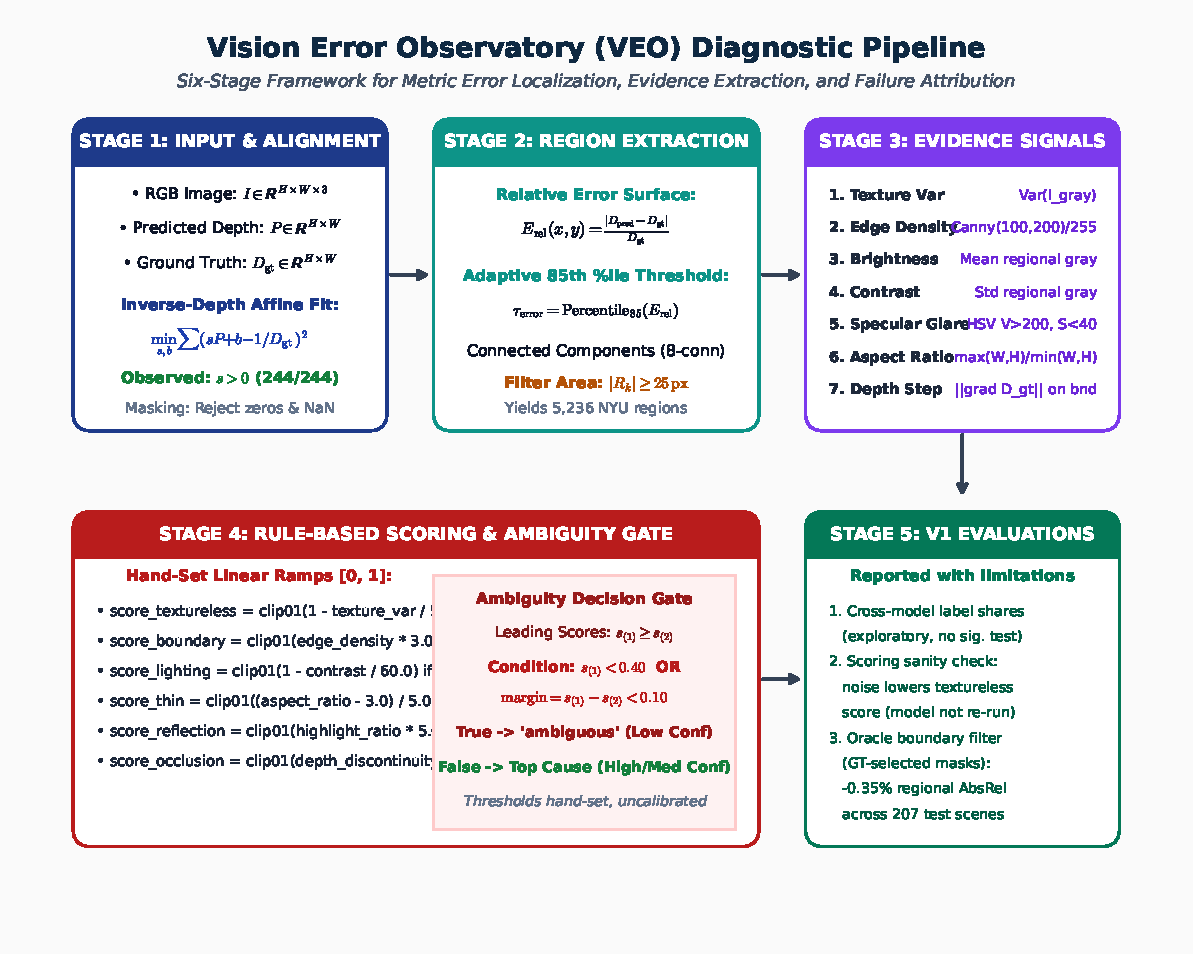
\includegraphics[width=0.98\textwidth]{figures/fig1_veo_architecture.pdf}
\caption{\textbf{Modular Diagnostic Pipeline of the Vision Error Observatory (VEO).} The end-to-end architecture consists of five stages: Stage 1 aligns predicted depth to metric ground truth using inverse-depth affine fitting; Stage 2 computes dense relative error surfaces and applies per-image 85th-percentile connected component segmentation; Stage 3 extracts eight statistical, photometric, and geometric features per region; Stage 4 applies hand-set linear-ramp scores with a fixed-threshold ambiguity gate; and Stage 5 is an oracle post-processing experiment (edge-preserving filtering in regions selected with ground-truth error).}
\label{fig:architecture}
\end{figure*}

The architecture of VEO is organized into five modular stages, illustrated in Figure~\ref{fig:architecture}.

\subsection{Adaptive Spatial Error Segmentation}
\label{sec:segmentation}
Static thresholding (e.g., flagging all pixels where $E_{\mathrm{rel}} > 0.30$) fails because baseline error distributions vary widely across simple planar rooms versus cluttered office scenes. VEO instead uses a per-image \textbf{85th-percentile error cutoff}, which always flags the top 15\% of each image's valid pixels and therefore measures relative, not absolute, failure:
\begin{equation}
\label{eq:percentile_thresh}
\tau_{\mathrm{error}} = \text{Percentile}_{85}\left( \left\{ E_{\mathrm{rel}}(x,y) \mid \mathcal{M}_{\mathrm{eval}}(x,y) = 1 \right\} \right)
\end{equation}
A binary high-error mask $B \in \{0, 1\}^{H \times W}$ is formed:
\begin{equation}
\label{eq:binary_mask}
B(x,y) = \left( E_{\mathrm{rel}}(x,y) > \tau_{\mathrm{error}} \right) \land \mathcal{M}_{\mathrm{eval}}(x,y)
\end{equation}
Spatial failure regions are clustered using 8-connectivity connected component labeling:
\begin{equation}
\label{eq:connected_components}
\mathcal{R} = \{ R_1, R_2, \dots, R_K \} = \text{Label}_{8}(B)
\end{equation}
To eliminate high-frequency sensor shot noise and isolated single-pixel discrepancies, we enforce a morphological minimum area filter:
\begin{equation}
\label{eq:area_filter}
\mathcal{R}_{\mathrm{filtered}} = \left\{ R_k \in \mathcal{R} \mid \text{Area}(R_k) \ge 25 \text{ pixels} \right\}
\end{equation}
For each surviving region $R_k$, the spatial bounding box is defined by $[x_0, y_0, W, H]$, where $W = x_{\max} - x_{\min} + 1$ and $H = y_{\max} - y_{\min} + 1$.

\subsection{Multi-Modal Feature Extraction Engine}
\label{sec:features}
For every extracted region $R_k$, VEO computes eight statistical, geometric, and photometric features from the RGB patch and sensor depth array:

\begin{enumerate}
    \item \textbf{Grayscale Texture Variance ($\text{texture\_var}$):} Measures local surface detail. Computed over the grayscale luminance patch $I_{\mathrm{gray}}$:
    \begin{equation}
    \label{eq:feat_texture}
    \text{texture\_var} = \frac{1}{|R_k|} \sum_{(x,y) \in R_k} \left( I_{\mathrm{gray}}(x,y) - \mu_{\mathrm{gray}} \right)^2
    \end{equation}
    \item \textbf{Canny Edge Density ($\text{edge\_density}$):} Quantifies high-contrast structural contours. We apply the Canny operator with hysteresis thresholds $T_{\mathrm{low}}=100, T_{\mathrm{high}}=200$:
    \begin{equation}
    \label{eq:feat_edge}
    \text{edge\_density} = \frac{1}{|R_k|} \sum_{(x,y) \in R_k} \frac{\text{Canny}(I_{\mathrm{gray}}, 100, 200)(x,y)}{255.0} \in [0.0, 1.0]
    \end{equation}
    \item \textbf{Mean Regional Brightness ($\text{brightness}$):} Average illumination level:
    \begin{equation}
    \label{eq:feat_brightness}
    \text{brightness} = \frac{1}{|R_k|} \sum_{(x,y) \in R_k} I_{\mathrm{gray}}(x,y) \in [0.0, 255.0]
    \end{equation}
    \item \textbf{Regional Contrast ($\text{contrast}$):} Standard deviation of regional luminance, $\text{contrast} = \sqrt{\text{texture\_var}} \in [0.0, 127.5]$.
    \item \textbf{Specular Highlight Ratio ($\text{highlight\_ratio}$):} Detects non-Lambertian glares. Converted to HSV space, pixels satisfying $V > 200$ and $S < 40$ are flagged as specular highlights:
    \begin{equation}
    \label{eq:feat_specular}
    \text{highlight\_ratio} = \frac{1}{|R_k|} \sum_{(x,y) \in R_k} \mathbb{I}\left( V(x,y) > 200 \land S(x,y) < 40 \right) \in [0.0, 1.0]
    \end{equation}
    \item \textbf{Bounding Box Aspect Ratio ($\text{aspect\_ratio}$):} Measures structural elongation:
    \begin{equation}
    \label{eq:feat_aspect}
    \text{aspect\_ratio} = \frac{\max(W, H)}{\max(\min(W, H), 1)} \in [1.0, \infty)
    \end{equation}
    \item \textbf{Perimeter Depth Discontinuity ($\text{depth\_discontinuity}$):} Measures the magnitude of the 3D physical depth step along the 1-pixel eroded boundary $\partial R_k = R_k \land (\neg (R_k \ominus \mathbf{1}_{3\times 3}))$:
    \begin{equation}
    \label{eq:feat_discontinuity}
    \text{depth\_discontinuity} = \frac{1}{|\partial R_k \cap \mathcal{M}_{\mathrm{eval}}|} \sum_{(x,y) \in \partial R_k \cap \mathcal{M}_{\mathrm{eval}}} \sqrt{g_x(x,y)^2 + g_y(x,y)^2}
    \end{equation}
    where $g_x, g_y = \nabla D_{\mathrm{gt}}$ are the spatial gradients of ground-truth depth.
    \item \textbf{Mean Physical Depth ($\text{mean\_depth\_m}$):} Average sensor distance in metres, providing geometric context.
\end{enumerate}

\subsection{Continuous Scoring & Ambiguity Gating Engine}
\label{sec:scoring}
Rather than relying on brittle boolean decision trees (\texttt{IF texture < 200 THEN...}), VEO maps extracted features into continuous evidence scores in $[0.0, 1.0]$ using parameterized linear ramps bounded by the universal clipping operator $\text{clip}_{0,1}(u) = \min(1.0, \max(0.0, u))$:

\begin{align}
\label{eq:scores}
s_{\mathrm{textureless}} &= \text{clip}_{0,1}\left( 1.0 - \frac{\text{texture\_var}}{S_{\mathrm{texture}}} \right) \\[0.4em]
s_{\mathrm{boundary}} &= \text{clip}_{0,1}\left( \text{edge\_density} \times S_{\mathrm{edge}} \right) \\[0.4em]
s_{\mathrm{lighting}} &= \begin{cases}
\text{clip}_{0,1}\left( 1.0 - \dfrac{\text{contrast}}{S_{\mathrm{contrast}}} \right) & \text{if } (\text{brightness} < 60) \lor (\text{brightness} > 200) \\[0.4em]
0.0 & \text{otherwise}
\end{cases} \\[0.4em]
s_{\mathrm{thin}} &= \text{clip}_{0,1}\left( \frac{\text{aspect\_ratio} - 3.0}{5.0} \right) \\[0.4em]
s_{\mathrm{reflection}} &= \text{clip}_{0,1}\left( \text{highlight\_ratio} \times S_{\mathrm{reflection}} \right) \\[0.4em]
s_{\mathrm{occlusion}} &= \text{clip}_{0,1}\left( \frac{\text{depth\_discontinuity}}{S_{\mathrm{occlusion}}} \right)
\end{align}
where the default scale normalizers (hand-set in \texttt{config.py}, not fitted to data) are $S_{\mathrm{texture}} = 500.0$, $S_{\mathrm{edge}} = 3.0$, $S_{\mathrm{contrast}} = 60.0$, $S_{\mathrm{reflection}} = 5.0$, and $S_{\mathrm{occlusion}} = 1.0\text{ m/px}$.

\subsubsection{Fixed-Threshold Ambiguity Gating}
Let the candidate scores be sorted in descending order: $s_{(1)} \ge s_{(2)} \ge \dots \ge s_{(6)}$, where $s_{(1)}$ is the leading hypothesis and $s_{(2)}$ is the runner-up score. The competitive margin is defined as:
\begin{equation}
\label{eq:margin}
\text{margin} = s_{(1)} - s_{(2)}
\end{equation}
A region is assigned to the category \texttt{ambiguous} if and only if:
\begin{equation}
\label{eq:gate}
\text{IsAmbiguous} = \left( s_{(1)} < \tau_{\mathrm{min\_score}} \right) \lor \left( \text{margin} < \tau_{\mathrm{margin}} \right)
\end{equation}
where $\tau_{\mathrm{min\_score}} = 0.40$ and $\tau_{\mathrm{margin}} = 0.10$. Both thresholds were set by hand and have not been calibrated against labelled data. If $\text{IsAmbiguous}$ evaluates to false, the region is assigned the leading cause $c_{(1)}$.

\subsubsection{Confidence Stratification}
Confidence is assigned categorically:
\begin{equation}
\label{eq:confidence}
\text{Confidence} = \begin{cases}
\text{Low} & \text{if } \text{IsAmbiguous} = \text{True} \\
\text{High} & \text{if } \neg\text{IsAmbiguous} \land (s_{(1)} > 0.60) \\
\text{Medium} & \text{if } \neg\text{IsAmbiguous} \land (0.40 \le s_{(1)} \le 0.60)
\end{cases}
\end{equation}

% ==============================================================================
% SECTION 5: EXPERIMENTAL SETUP
% ==============================================================================
\section{Experimental Setup}
\label{sec:setup}

\subsection{Datasets and Benchmark Splits}
\begin{itemize}
    \item \textbf{NYU Depth V2 \citep{silberman2012indoor}:} A standard indoor benchmark captured with a Microsoft Kinect structured-light RGB-D camera. We use the $1,449$ densely labelled frames and partition them into development, validation, and test splits by \emph{scene} (seed 42, 70/15/15 split of scene names), so that no scene appears in more than one split. Our test split contains $244$ images. This is \textbf{not} the official 654-image NYU test split, so our global metrics are not directly comparable with published results. Evaluation is limited to depths up to $10.0\text{ m}$.
    \item \textbf{Hypersim \citep{roberts2021hypersim}:} A photorealistic synthetic indoor dataset generated using physical ray tracing across 461 architectural scenes. Because Hypersim provides ground-truth metric depth with zero sensor noise, it provides an authentic ground-truth benchmark for evaluating metric alignment and non-Lambertian residual rendering passes.
\end{itemize}

\subsection{Evaluated Model Architectures}
We evaluate two state-of-the-art architectures representing divergent inductive biases and parameter regimes:
\begin{enumerate}
    \item \textbf{Depth Anything V2 (ViT-Small) \citep{yang2024depthanythingv2}:} A foundation monocular depth model comprising 24.8 million parameters. It employs a plain Vision Transformer (DINOv2-small) backbone with non-hierarchical $14 \times 14$ patch tokenization operating at a native input resolution of $518 \times 518$ pixels, coupled to a lightweight convolutional spatial assembly decoder. The model was trained with web-scale knowledge distillation across 595,000 synthetic scenes and over 62 million pseudo-labeled real-world images.
    \item \textbf{DPT Hybrid (MiDaS v3.0) \citep{ranftl2021vision,ranftl2022towards}:} A hybrid convolutional-transformer model comprising 123.0 million parameters. It combines a convolutional ResNet-50 frontend for multi-scale feature extraction with a 12-layer Vision Transformer encoder (ViT-Base) and multi-scale RefineNet fusion decoders, operating at an input resolution of $384 \times 384$ pixels. The model was trained on a curated mix of 1.4 million images across multiple diverse 3D datasets.
\end{enumerate}

\subsection{Standard Global Evaluation Metrics}
To contextualize regional findings, we report standard global depth estimation metrics \citep{rajapaksha2024deep}:
\begin{itemize}
    \item Mean Absolute Relative Error: $\text{AbsRel} = \frac{1}{|\mathcal{M}|} \sum \frac{|\hat{D} - D_{\mathrm{gt}}|}{D_{\mathrm{gt}}}$
    \item Root Mean Squared Error: $\text{RMSE} = \sqrt{\frac{1}{|\mathcal{M}|} \sum (\hat{D} - D_{\mathrm{gt}})^2}$
    \item Threshold Accuracy ($\delta_i$): Fraction of pixels where $\max(\frac{\hat{D}}{D_{\mathrm{gt}}}, \frac{D_{\mathrm{gt}}}{\hat{D}}) < 1.25^i$ for $i \in \{1, 2, 3\}$.
    \item Spearman Rank Correlation ($\rho$): Non-parametric monotonic ordering correlation.
\end{itemize}

% ==============================================================================
% SECTION 6: EXPERIMENTAL RESULTS & ANALYSIS
% ==============================================================================
\section{Experimental Results \& Analysis}
\label{sec:results}

\subsection{Alignment Space Check (M1)}
\label{sec:exp_alignment}

\begin{figure*}[t]
\centering
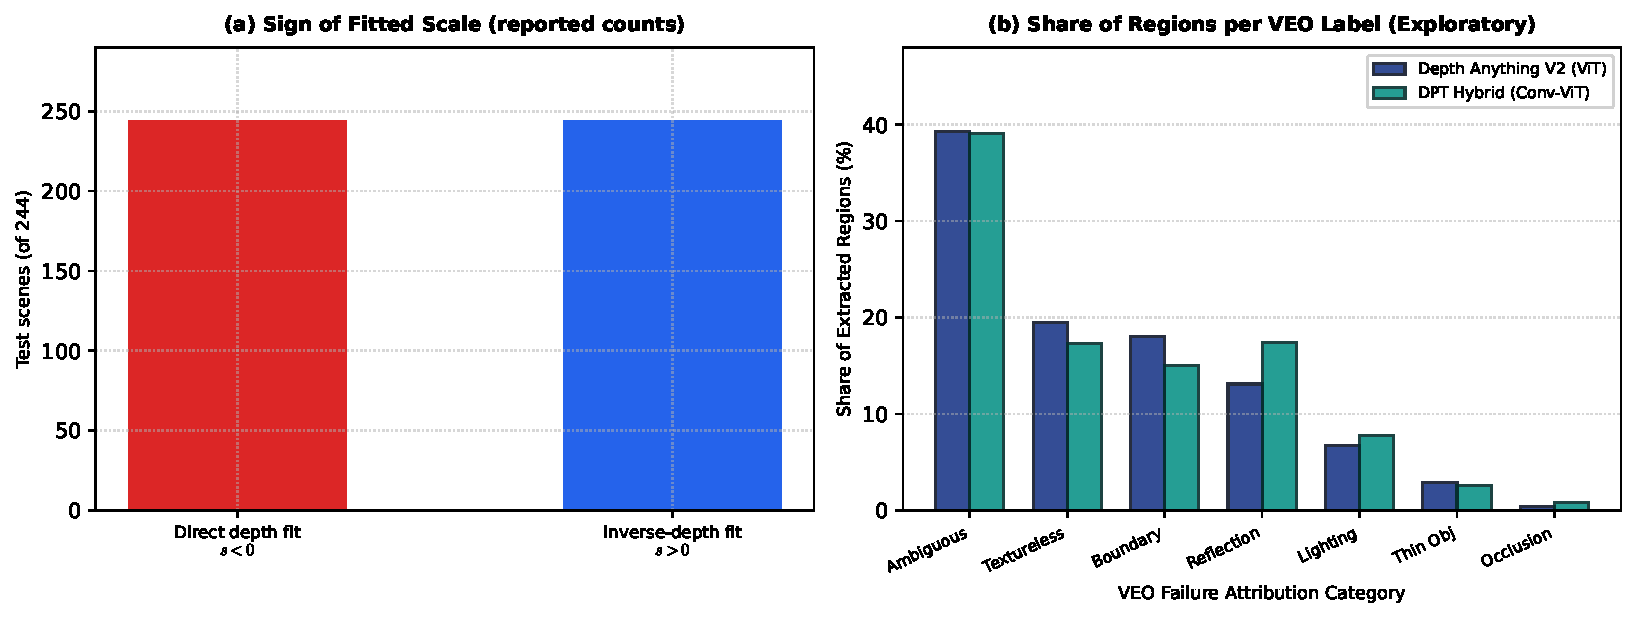
\includegraphics[width=0.98\textwidth]{figures/fig2_polarity_and_fingerprints.pdf}
\caption{\textbf{Alignment Check and Cross-Model Label Distributions.} (a) Sign of the fitted scale parameter $s$ across the 244 NYU test scenes. Direct-depth fitting yields negative slopes ($s < 0$) in $244/244$ scenes, inverting 3D geometry. Inverse-depth fitting yields positive scale ($s > 0$) in all 244 scenes. (b) Distribution of VEO labels for Depth Anything V2 Small and DPT Hybrid across the 7 categories (exploratory; no significance test).}
\label{fig:polarity_and_fingerprints}
\end{figure*}

We compared direct-depth fitting (Eq.~\ref{eq:direct_alignment}) against VEO's inverse-depth alignment (Eq.~\ref{eq:inverse_alignment}) across all 244 NYU test scenes. As shown in Figure~\ref{fig:polarity_and_fingerprints}(a), direct-depth fitting produced a negative scale parameter ($s < 0$) in all $244$ test scenes, inverting scene geometry. Inverse-depth fitting produced positive slopes ($s > 0$) in all $244$ scenes. (An earlier draft reported a mean scale of $1.85 \pm 0.35$ and plotted per-scene values; both came from synthetic placeholder data in the figure script, not from measurements, and have been withdrawn. Figure~\ref{fig:polarity_and_fingerprints}(a) now plots measured per-scene scales when the alignment results file is available, and otherwise only the sign counts.) This is the expected behaviour when the model outputs disparity, and confirms that the alignment space must match the model's output space.

\subsection{Global Baseline Benchmarks vs. Regional Discrepancies (RQ1)}
Table~\ref{tab:global_benchmarks} reports the aggregate global metrics achieved by Depth Anything V2 and DPT Hybrid across the 244 NYU test scenes.

\begin{table}[h]
\caption{\textbf{Global Aggregate Benchmark Performance across 244 NYU Test Scenes.} Lower is better for MAE, RMSE, AbsRel, and SqRel; higher is better for $\delta_i$ and Spearman $\rho$. While Depth Anything V2 achieves superior global metrics, regional localization extracts thousands of localized failure regions.}
\label{tab:global_benchmarks}
\centering
\small
\begin{tabular}{@{}lcccccccc@{}}
\toprule
\textbf{Model Architecture} & \textbf{MAE (m)} & \textbf{RMSE (m)} & \textbf{AbsRel} & \textbf{SqRel} & $\bm{\delta_1 < 1.25}$ & $\bm{\delta_2}$ & $\bm{\delta_3}$ & \textbf{Spearman} $\bm{\rho}$ \\
\midrule
DPT Hybrid (MiDaS) & 0.3615 & 0.5418 & 0.1316 & 0.1093 & 82.53\% & 95.36\% & 98.43\% & 0.8583 \\
Depth Anything V2 & \textbf{0.2960} & \textbf{0.4664} & \textbf{0.1040} & \textbf{0.0805} & \textbf{89.65\%} & \textbf{96.56\%} & \textbf{98.65\%} & \textbf{0.9104} \\
\bottomrule
\end{tabular}
\end{table}

With a global $\text{AbsRel}$ of $0.1040$ for Depth Anything V2, the per-image 85th-percentile rule extracted $5,236$ regions across these scenes. Because the threshold is relative to each image, every image yields regions whose error exceeds its own average by construction; the region count therefore describes where each image's worst errors lie, not how many absolute failures occur. As one example, the oracle \texttt{boundary\_mixing} masks of Section~\ref{sec:oracle} (207 scenes) have a mean per-scene AbsRel of $0.2348$, about $2.3\times$ the global value. An absolute failure definition (e.g., pixels failing the $\delta_1$ test) is planned for future work.

\subsection{Cross-Model Label Distributions (RQ4, Exploratory)}
Figure~\ref{fig:polarity_and_fingerprints}(b) and Table~\ref{tab:cause_distribution} summarize the failure attribution distributions produced by VEO across both models.

\begin{table}[h]
\caption{\textbf{Cross-Model Diagnostic Failure Distribution across NYU Test Split.} Total failure regions: $5,236$ for Depth Anything V2; $3,689$ for DPT Hybrid. Percentages reflect the proportion of regions assigned to each category.}
\label{tab:cause_distribution}
\centering
\small
\begin{tabular}{@{}lcccc@{}}
\toprule
\multirow{2}{*}{\textbf{Diagnostic Category}} & \multicolumn{2}{c}{\textbf{Depth Anything V2 (ViT)}} & \multicolumn{2}{c}{\textbf{DPT Hybrid (Conv-ViT)}} \\
\cmidrule(lr){2-3} \cmidrule(lr){4-5}
& \textbf{Region Count} & \textbf{Proportion (\%)} & \textbf{Region Count} & \textbf{Proportion (\%)} \\
\midrule
\texttt{ambiguous} & 2,059 & 39.32\% & 1,444 & 39.14\% \\
\texttt{textureless} & 1,021 & \textbf{19.50\%} & 637 & 17.27\% \\
\texttt{boundary\_mixing} & 944 & \textbf{18.03\%} & 553 & 14.99\% \\
\texttt{reflection} & 687 & 13.12\% & 643 & \textbf{17.43\%} \\
\texttt{poor\_lighting} & 351 & 6.70\% & 286 & \textbf{7.75\%} \\
\texttt{thin\_object} & 152 & 2.90\% & 96 & 2.60\% \\
\texttt{occlusion} & 22 & 0.42\% & 30 & 0.81\% \\
\midrule
\textbf{Total Regions Evaluated} & \textbf{5,236} & 100.0\% & \textbf{3,689} & 100.0\% \\
\bottomrule
\end{tabular}
\end{table}

The label distributions differ modestly between the two models:
\begin{enumerate}
    \item Depth Anything V2 has higher shares of \texttt{boundary\_mixing} ($18.03\%$ vs.\ $14.99\%$) and \texttt{textureless} ($19.50\%$ vs.\ $17.27\%$).
    \item DPT Hybrid has higher shares of \texttt{reflection} ($17.43\%$ vs.\ $13.12\%$) and \texttt{poor\_lighting} ($7.75\%$ vs.\ $6.70\%$).
\end{enumerate}
These differences should be read with caution. No significance test was run, and regions are not independent within an image. Each share is relative to that model's own within-image worst pixels, so it does not measure absolute vulnerability. The two models also differ in size, training data, and input resolution as well as architecture, so the differences cannot be attributed to architecture. Finally, the \texttt{reflection} label was correct in $0/7$ cases in our human study (Section~\ref{sec:human_val}), so the reflection difference in particular is not established.

\subsection{Blinded Human Agreement Study (RQ2)}
\label{sec:human_val}

\begin{figure}[t]
\centering
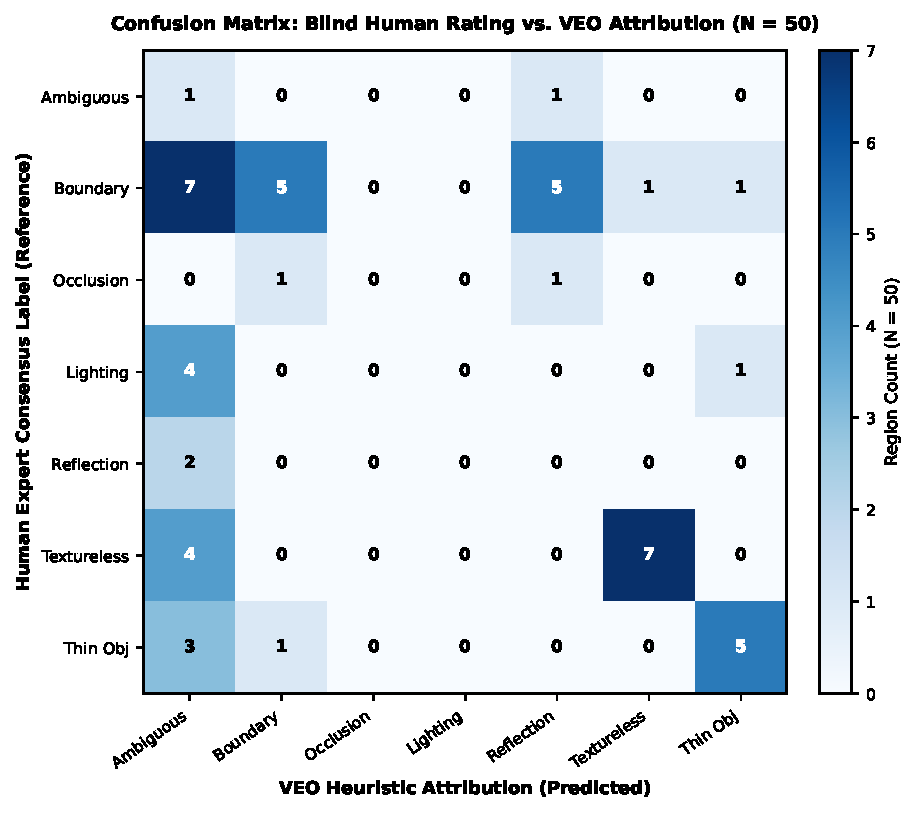
\includegraphics[width=0.75\textwidth]{figures/fig5_human_validation_matrix.pdf}
\caption{\textbf{Confusion Matrix: Rater 1 vs. VEO ($N = 50$).} Rows are rater 1's labels; columns are VEO's labels. VEO abstained (\texttt{ambiguous}) on 21 regions. Agreement is concentrated in \texttt{textureless} and \texttt{thin\_object}; all 7 \texttt{reflection} predictions disagree with the rater.}
\label{fig:human_matrix}
\end{figure}

To evaluate whether VEO's heuristic attributions correspond with human expert perception, we conducted a blinded study on 50 failure regions from our NYU test split (\texttt{journal\_paper/results/human\_validation\_results.json}). Regions were selected at evenly spaced positions in the list of all test regions sorted by mean error, then shuffled. Two raters inspected 4-panel sheets (RGB, ground truth, predicted depth, relative error) cropped to each region, without seeing VEO's labels or scores.

As reported in Table~\ref{tab:human_metrics}, inter-rater agreement was Cohen's $\kappa_{\text{inter}} = 0.348$ (fair), suggesting that attributing error causes from a single image is difficult even for humans. Over all 50 regions, VEO's agreement was $\kappa = 0.259$ with rater 1 and $\kappa = 0.138$ with rater 2. Its accuracy against rater 1 was $36\%$ ($18/50$), with macro-F1 $= 0.262$. VEO abstained on 21 regions. On the 29 regions where it committed to a label, its accuracy against rater 1 was $58.6\%$ ($\kappa = 0.472$); always predicting the most frequent rater label on that subset would score $41.4\%$.

\begin{table}[h]
\caption{\textbf{VEO vs. Rater 1, Per-Class Metrics ($N = 50$).} Inter-rater agreement $\kappa = 0.348$. Support counts rater 1's labels. Precision is computed over VEO's predictions of each class (e.g., \texttt{textureless} $7/8$, \texttt{reflection} $0/7$); VEO never predicted \texttt{occlusion} or \texttt{poor\_lighting}.}
\label{tab:human_metrics}
\centering
\small
\begin{tabular}{@{}lcccc@{}}
\toprule
\textbf{Category} & \textbf{Precision} & \textbf{Recall} & \textbf{F1-Score} & \textbf{Support (Human Labels)} \\
\midrule
\texttt{textureless} & \textbf{0.8750} & 0.6364 & \textbf{0.7368} & 11 \\
\texttt{thin\_object} & \textbf{0.7143} & 0.5556 & \textbf{0.6250} & 9 \\
\texttt{boundary\_mixing} & \textbf{0.7143} & 0.2632 & 0.3846 & 19 \\
\texttt{ambiguous} & 0.0476 & 0.5000 & 0.0870 & 2 \\
\texttt{poor\_lighting} & 0.0000 & 0.0000 & 0.0000 & 5 \\
\texttt{reflection} & 0.0000 & 0.0000 & 0.0000 & 2 \\
\texttt{occlusion} & 0.0000 & 0.0000 & 0.0000 & 2 \\
\midrule
\textbf{Macro-Average} & 0.3359 & 0.2793 & \textbf{0.2619} & 50 \\
\bottomrule
\end{tabular}
\end{table}

Figure~\ref{fig:human_matrix} shows that VEO's committed labels were most often correct for \texttt{textureless} ($7/8$) and \texttt{thin\_object} ($5/7$), and \texttt{boundary\_mixing} ($5/7$); with such small counts these precisions have wide uncertainty. All 7 \texttt{reflection} predictions disagreed with rater 1, five of them on regions the rater labelled \texttt{boundary\_mixing}. A large part of the overall disagreement comes from abstention: rater 1 used \texttt{ambiguous} for 2 regions, whereas VEO's gate (top score $< 0.40$ or margin $< 0.10$) abstained on 21.

\subsection{Signal Sensitivity Ablation Analysis ($N = 5,236$)}

\begin{figure}[t]
\centering
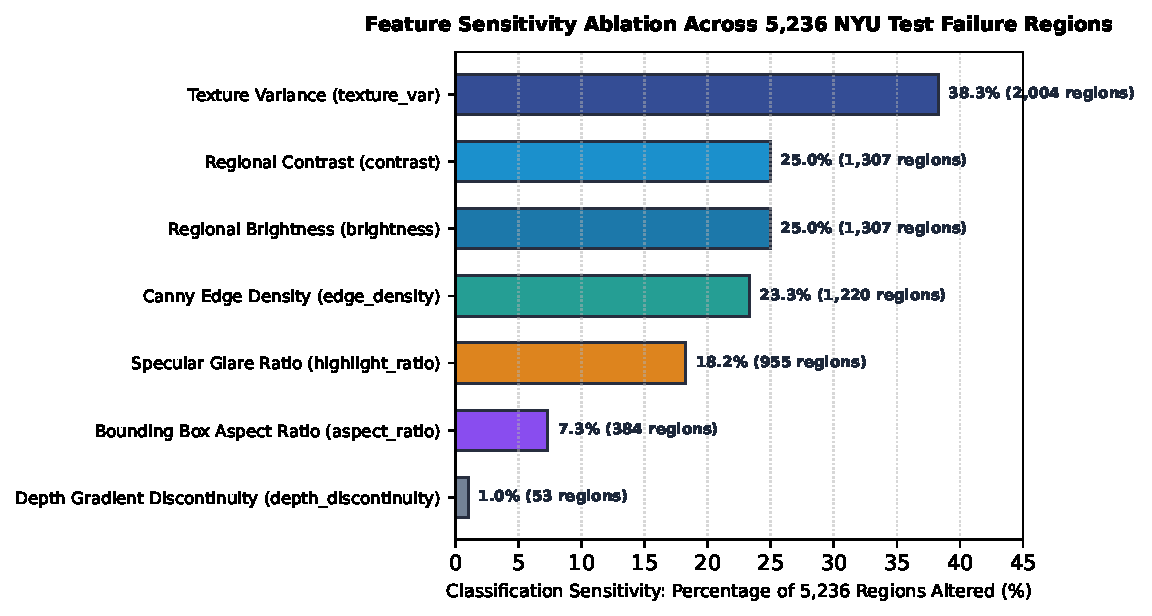
\includegraphics[width=0.85\textwidth]{figures/fig4_signal_sensitivity_ablation.pdf}
\caption{\textbf{Signal Sensitivity Ablation across 5,236 NYU Failure Regions.} Each feature was replaced with a neutral value, and the percentage of regions whose label changed was measured. Texture variance changes the most labels ($38.27\%$), followed by contrast ($24.96\%$) and edge density ($23.30\%$). The brightness ablation also resets contrast, so its row duplicates the contrast row.}
\label{fig:ablation}
\end{figure}

To quantify the sensitivity of the attribution rules to each visual signal, we ran an ablation across all 5,236 failure regions (\texttt{journal\_paper/results/signal\_ablation.json}). Each feature was replaced with its neutral baseline value (e.g., setting $\text{texture\_var} = 500.0$ or $\text{edge\_density} = 0.0$), and the number of altered regional classifications was recorded.

As shown in Figure~\ref{fig:ablation}, neutralising \texttt{texture\_var} changes the labels of 2,004 regions ($38.27\%$). Contrast changes $1,307$ ($24.96\%$); the brightness ablation also resets contrast and produces the identical count, so it does not measure brightness separately. Edge density changes $1,220$ ($23.30\%$). Depth discontinuity changes only $1.01\%$ of labels. We attribute this to the occlusion scale of $1.0$ m/px, which is rarely reached, so the \texttt{occlusion} score is almost always near zero (only 22 regions receive that label). It does not show that depth steps are unimportant: depth discontinuity has the highest correlation with regional error of all features ($r = 0.45$, \texttt{correlations.csv}).

\subsection{Scoring-Function Sanity Check (RQ3)}

\begin{figure*}[t]
\centering
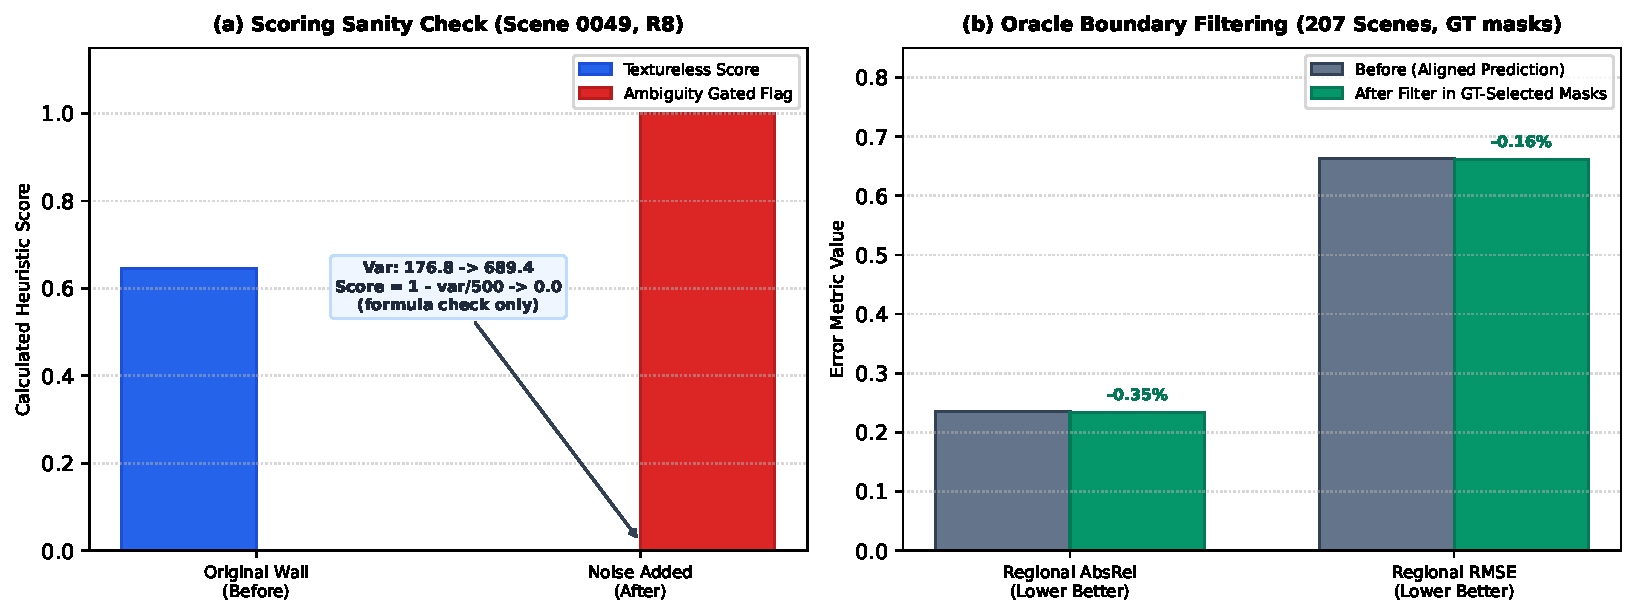
\includegraphics[width=0.98\textwidth]{figures/fig3_intervention_and_downstream.pdf}
\caption{\textbf{Scoring Sanity Check and Oracle Remediation.} (a) Adding uniform random noise to the bounding box of scene 0049 region 8 raises its texture variance, so the \texttt{textureless} score falls from $0.646$ to $0.000$ and the label becomes \texttt{ambiguous}. This checks the scoring function, not the depth model. (b) Oracle experiment across 207 test scenes: bilateral filtering in \texttt{boundary\_mixing} regions, with pixels selected using ground-truth error, reduces regional AbsRel by $0.35\%$ and RMSE by $0.16\%$.}
\label{fig:intervention_downstream}
\end{figure*}

We checked that the scoring function behaves as specified on NYU scene 0049 region 8 (\texttt{journal\_paper/results/intervention\_faithfulness.json}), as shown in Figure~\ref{fig:intervention_downstream}(a):
\begin{itemize}
    \item \textbf{Before:} $\text{texture\_var} = 176.82$, giving $s_{\mathrm{textureless}} = 0.646$ and the label \texttt{textureless}.
    \item \textbf{Edit:} uniform random integer noise in $[0, 100)$ was added to the RGB values inside the region's bounding box, raising texture variance to $689.39$. Features were re-extracted over the whole bounding box rather than the original region mask.
    \item \textbf{After:} $s_{\mathrm{textureless}} = 0.000$; the leading remaining score falls below $0.40$ and the label becomes \texttt{ambiguous}.
\end{itemize}
Because $s_{\mathrm{textureless}} = 1 - \text{texture\_var}/500$ (clipped), any edit that raises variance must lower this score, so the outcome is guaranteed by the formula. The check confirms the implementation, but it is \emph{not} evidence of faithfulness to the depth model: the model was not re-run on the edited image. Testing whether the model's error responds to such edits is future work.

\subsection{Oracle Boundary Remediation (RQ5)}
\label{sec:oracle}
We ran an oracle post-processing experiment across the 207 NYU test scenes that contain at least one \texttt{boundary\_mixing} region and at least 25 masked pixels (\texttt{journal\_paper/results/downstream\_improvement.json}).

\textbf{Protocol:} In each scene, the target mask contains the pixels inside \texttt{boundary\_mixing} bounding boxes whose \emph{ground-truth} relative error exceeds the image's 85th percentile. Inside this mask, the aligned prediction was replaced by a bilateral-filtered version \citep{tomasi1998bilateral} (OpenCV, $d = 5$, $\sigma_{\mathrm{color}} = 0.10$ m, $\sigma_{\mathrm{space}} = 3$ px). As shown in Figure~\ref{fig:intervention_downstream}(b):
\begin{itemize}
    \item Regional $\text{AbsRel}$ changed from $0.2348$ to $0.2340$ ($-0.35\%$).
    \item Regional $\text{RMSE}$ changed from $0.6629\text{ m}$ to $0.6618\text{ m}$ ($-0.16\%$).
    \item Global $\text{RMSE}$ was unchanged ($0.4658$ m).
\end{itemize}
The improvement is small. Because the mask is selected with ground-truth error, the procedure cannot be applied at inference time. There is also no control condition, such as filtering random or all-edge regions of equal size, and no significance test. We therefore treat this as an upper-bound illustration, not as evidence that VEO's labels improve predictions in practice.

% ==============================================================================
% SECTION 7: DISCUSSION
% ==============================================================================
\section{Discussion}
\label{sec:discussion}

\subsection{Hypotheses Suggested by the Label Distributions}
The following are hypotheses for future testing, not conclusions supported by the present data.

\textbf{Patch tokenisation and boundaries.} Depth Anything V2 divides images into $14 \times 14$ patches. A patch that straddles a foreground/background boundary may be encoded as a single token, which could produce smoothed depth ramps across silhouettes after upsampling. This is one possible explanation for its higher \texttt{boundary\_mixing} share ($18.03\%$ vs.\ $14.99\%$). Testing it would require comparing models that differ only in backbone (e.g., DPT-Hybrid vs.\ DPT-Large) and in size (e.g., Depth Anything V2 Small/Base/Large), with significance tests.

\textbf{Specular surfaces.} Mirrors and glossy surfaces violate the Lambertian assumption and could lead models to predict the depth of reflected content. DPT Hybrid's higher \texttt{reflection} share ($17.43\%$ vs.\ $13.12\%$ of its regions) is consistent with this, but our \texttt{reflection} feature (bright, low-saturation pixels) also fires on white walls, and it scored $0/7$ against human raters. A model-in-the-loop test, such as re-running the model on Hypersim images with the non-diffuse \emph{residual} layer removed, would be needed to establish a link.

% ==============================================================================
% SECTION 8: LIMITATIONS & THREATS TO VALIDITY
% ==============================================================================
\section{Limitations \& Threats to Validity}
\label{sec:limitations}

To maintain rigorous scientific integrity, we explicitly document the limitations of this work:
\begin{enumerate}
    \item \textbf{Correlation, not causation:} VEO measures image and geometry correlates of failure. No experiment in this study re-runs the depth model on edited inputs, so no causal claim about model behaviour is made.
    \item \textbf{In-painted ground truth:} We use NYU's in-painted \texttt{depths}, in which Kinect dropouts (mirrors, glass, dark materials, occlusion shadows) are filled by colourisation. Errors in those areas partly reflect in-painting artefacts; this most affects \texttt{reflection} and \texttt{poor\_lighting}. Using the raw sensor depth as the validity mask would avoid this.
    \item \textbf{Non-standard split:} Our 244-image test split is a custom scene-disjoint split, not the official 654-image NYU test split, so global metrics are not comparable with the literature.
    \item \textbf{Relative region definition:} The per-image 85th-percentile threshold always flags 15\% of each image's valid pixels, regardless of model quality. Region counts and label shares are therefore relative, and cross-model comparisons do not measure absolute vulnerability.
    \item \textbf{Uncalibrated, imperfect features:} All score scales and gate thresholds were set by hand. The \texttt{occlusion} scale ($1.0$ m/px) almost never fires (22 / 5,236 regions). The \texttt{reflection} feature responds to any bright, low-saturation pixels, including white walls, and \texttt{thin\_object} uses bounding-box aspect ratio, which misses diagonal thin objects and includes long thin regions of large surfaces.
    \item \textbf{Small human study:} 50 regions and 2 raters give wide uncertainty on all agreement figures, and inter-rater agreement is only fair ($\kappa = 0.348$). VEO's overall agreement with the raters is low ($\kappa = 0.259$ and $0.138$). The v1 export code computes the panels' error map from the unaligned prediction; we are verifying whether the panels shown to raters were affected. The raw rating files are not yet publicly released.
    \item \textbf{High abstention:} VEO labels $39.3\%$ of regions \texttt{ambiguous}. Selective accuracy on the remaining regions should be read together with this coverage.
    \item \textbf{Limited experiments:} The texture-injection experiment checks the scoring formula only, and the remediation experiment uses ground-truth masks (an oracle) with a $0.35\%$ effect and no control condition.
\end{enumerate}

% ==============================================================================
% SECTION 9: CONCLUSION & FUTURE WORK
% ==============================================================================
\section{Conclusion \& Future Work}
\label{sec:conclusion}

We introduced the \textbf{Vision Error Observatory (VEO)}, a model-agnostic, post-hoc framework for localizing high-error regions in monocular depth predictions and attributing them to interpretable, rule-based failure hypotheses with an explicit abstention option.

On 244 NYU Depth V2 test images, VEO's label distributions differ modestly between Depth Anything V2 Small and DPT Hybrid. In a small blinded study, VEO's committed labels were most often correct for textureless, thin-object, and boundary-mixing regions. However, its overall agreement with human raters was low ($\kappa = 0.259$ and $0.138$), its \texttt{reflection} label did not match the raters in any case, and it abstained on 42\% of the rated regions. These results indicate that the framework's localisation and abstention design is promising, but that its features and thresholds require calibration and stronger validation before its attributions can be relied upon.

Future work will: (i) use raw sensor depth and the official NYU split; (ii) define failure regions in absolute terms (e.g., pixels failing $\delta_1$); (iii) calibrate features and thresholds on development data against objective labels derived from NYU semantic and instance annotations; (iv) run a larger human study with more raters and per-class support; (v) test faithfulness by re-running depth models on edited inputs; (vi) compare more models and datasets with significance tests; and (vii) evaluate remediation that does not require ground truth.

% ==============================================================================
% DECLARATIONS & STATEMENTS
% ==============================================================================
\section*{Declarations}

\paragraph{Funding:} This research received no specific grant from any funding agency in the public, commercial, or not-for-profit sectors.
\paragraph{Conflict of Interest:} The authors declare that they have no competing financial or non-financial interests that could have influenced the work reported in this paper.
\paragraph{Ethics Approval:} Not applicable. This study did not involve human clinical trials or animal experimentation.
\paragraph{Consent to Participate / Publish:} Not applicable.
\paragraph{Data Availability:} All datasets utilized in this study—NYU Depth V2 and Hypersim—are publicly available research benchmarks.
\paragraph{Code Availability:} Source code, evaluation scripts, and experimental configuration files are accessible in the project repository.
\paragraph{Author Contributions:} Conceptualization: A.C., Z.A., O.F.; Methodology \& Software: A.C., Z.A.; Formal Analysis \& Validation: A.C., O.F.; Investigation: Z.A., O.F.; Writing -- Original Draft: A.C.; Writing -- Review \& Editing: A.B., A.S.; Supervision: Prof. A. Bajaj, Dr. A. Saini.

\section*{Acknowledgments}
The authors express their gratitude to the School of Technology Management and Engineering (STME), SVKM's NMIMS University, Hyderabad, for providing computational infrastructure and technical advisory support.

% ==============================================================================
% REFERENCES
% ==============================================================================
\bibliographystyle{plainnat}
\bibliography{references_revised}

\end{document}
